\section{PN Diode and Zener Diode in Circuit}

\subsection{Introduction}
    \subsubsection{Background}
    Diode are electronic componet made from semiconductor material. It is a two-terminal device that allows current to flow in one direction only.\par

    In this experiment, we want to analyze the properties of diodes in circuits. We will use a pn diode, a Schottky diode, and a zener diode to construct simple circuits and verify their performance.\par

    \subsubsection{Propose}
    \begin{itemize}
        \item To learn the basic property of a pn diode and a zener diode
        \item To construct simple circuits and verify their performance
    \end{itemize}

    \subsubsection{Theory}
    The three diode have different characteristics, and need to be threated differently in the circuit.\par
    \begin{itemize}
        \item \textbf{Regular PN Diode}
            This kind of diode have two working mode, and is determined by the voltage applied across it. 
            \begin{enumerate}
                \item \textbf{Forward Active}\newline
                    When the voltage across the diode is greater than the build in voltage $V_{\gamma}$, the diode is on and the current can flow through it. $V_{\gamma}$ is usually $0.7V$.
                \item \textbf{Reverse Active}\newline
                    When the voltage across the diode is smaller than $V_{\gamma}$, the diode is off and the current can not flow through it.
            \end{enumerate}
    
        \item \textbf{Schottky Diode}
            This kind of diode is similar to regular diode, but has a lower forward voltage drop and faster switching speed. Its working modes also determined by the voltage applied across it.
            \begin{enumerate}
                \item \textbf{Forward Active}\newline
                    When the voltage across the diode exceeds the forward voltage $V_{\gamma}$, the diode turns on and allows current to flow. For Schottky diodes, $V_{\gamma}$ is typically between $0.2V$ and $0.3V$, which is lower than that of a regular PN diode.

                \item \textbf{Reverse Active}\newline
                    When the voltage across the diode is less than $V_{\gamma}$, the diode is off. Different from regular diode, Schottky diodes generally have some noticeable reverse current when reverse biased.
            \end{enumerate}
        
        \item \textbf{Zener Diode}
            This type of diode is specifically designed to work in reverse breakdown mode, and it can limit the voltage across it in the breakdown mode. Its working modes are:
            \begin{enumerate}
                \item \textbf{Forward Active}\newline
                    When the voltage across the diode exceeds the forward voltage $V_{\gamma}$, typically around $0.7V$, the Zener diode behaves like a regular PN diode and allows current to flow.

                \item \textbf{Reverser Active}\newline
                    When the voltage across the diode less than the forward voltage $V_{\gamma}$, and yet didn't exceed the Zener breakdown voltage $V_Z$, the diode is off like regular diode, and no current flows through it.

                \item \textbf{Reverse Breakdown}\newline
                    When the reverse voltage across the diode exceeds its Zener breakdown voltage $V_Z$, the diode breakdown, and limit the voltage across it to $V_Z$.
            \end{enumerate}
    \end{itemize}
\subsection{Experiment Design}
    \subsubsection{Materials}
        In this experiment, we will use the following components:
        \begin{itemize}
            \item 1N4148 Diode
            \item SR160 Schottky didode
            \item 1N4728A Zener diode
            \item Resistors
            \item Breadboard
            \item DC Power Supply
            \item Digital Multimeter
        \end{itemize}

    \subsubsection{Circuit Diagram}
        The following circuit diagrams is used in our experiment.
        \begin{figure}[H]
            \centering
            \begin{subfigure}{0.4\textwidth}
                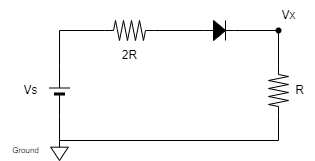
\includegraphics[width=1\linewidth]{Experiment_01/Circuit/Lab1a.png}
                \caption{ }
                \label{cir:1a}
            \end{subfigure}
            \begin{subfigure}{0.4\textwidth}
                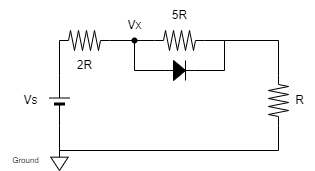
\includegraphics[width=1\linewidth]{Experiment_01/Circuit/Lab1b.png}
                \caption{ }
                \label{cir:1b}
            \end{subfigure}

            \begin{subfigure}{0.4\textwidth}
                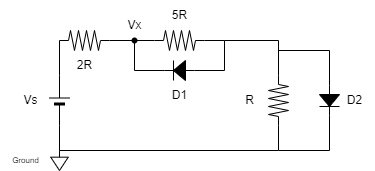
\includegraphics[width=1\linewidth]{Experiment_01/Circuit/Lab1c.png}
                \caption{ }
                \label{cir:1c}
            \end{subfigure}
            \begin{subfigure}{0.4\textwidth}
                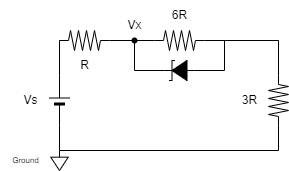
\includegraphics[width=1\linewidth]{Experiment_01/Circuit/Lab1d.png}
                \caption{ }
                \label{cir:1d}
            \end{subfigure}
            \caption{Simple Diode Circuit}
        \end{figure}

    \subsubsection{Theoretical Analysis}
        \begin{enumerate}[a]
            \item \textbf{Circuit in figure \ref{cir:1a}}\newline
                The circuit in figure \ref{cir:1a} is a simple diode circuit. The diode is forward biased when the $V_S$ is greater than $V_{\gamma}$. Other wise the diode will not conduct. 
                \begin{itemize}
                \item \textbf{Forward active}\newline
                    When forward active, the voltage across the diode is $V_{\gamma}$, and we can write the KVL:
                    \begin{equation}
                        V_S = V_{\gamma} + I(2R) + IR
                    \end{equation}
                    Re arrange the equation, we have:
                    \begin{equation}
                        I = \frac{V_S - V_{\gamma}}{3R}
                    \end{equation}
                    According to the Ohm's law, the voltage $V_X$ across the resistor R can be calulated as:
                    \begin{equation}
                        V_X = IR = \frac{2}{3}(V_S - V_{\gamma})
                    \end{equation}
                \item \textbf{Reverse active}\newline
                    When reverse active, the diode is off, and there will be no current in the circuit. So the voltage $V_X$ across the resistor R is 0.
                \end{itemize}
                Cobine the two conditions, we have the function of the voltage $V_X$ across the resistor R with respect to the input voltage $V_S$:
                \begin{equation}
                    \begin{cases}
                        V_x = \frac{2}{3}V_s - V_\gamma & V_s \ge V_\gamma\\
                        V_x = 0 & V_s < V_\gamma\\
                    \end{cases}
                \label{eq:1a}
                \end{equation}
                where $I_s$ is the reverse saturation current, $V$ is the voltage across the diode, $n$ is the ideality factor, and $V_T$ is the thermal voltage.

            \item \textbf{Circuit in figure \ref{cir:1b}}\newline
                Similarly, by discuss the situation in the circuit seperatly in difference operation mode, we can get the function of the voltage $V_X$ across the resistor R with respect to the input voltage $V_S$:
                \begin{equation}
                    \begin{cases}
                        V_x = \frac{V_s+2V_\gamma}{3} & V_s\ge \frac{8}{5}V_\gamma\\
                        V_x = \frac{3V_s}{4} & V_s < \frac{8}{5}V_\gamma\\
                    \end{cases}
                \label{eq:1b}
                \end{equation}

            \item \textbf{Circuit in figure \ref{cir:1c}}\newline
                Apply the same method, we can get the function of the voltage $V_X$ across the resistor R with respect to the input voltage $V_S$:
                \begin{equation}
                    \begin{cases}
                        V_x = \frac{5V_s+2V_\gamma}{7} 
                        & V_s \in (8V_\gamma,~\inf)\\

                        V_x = \frac{3V_s}{4} 
                        & V_s \in (-\frac{8}{5}V_\gamma,~8V_\gamma]\\

                        V_x = \frac{V_s-2V_\gamma}{3} 
                        & V_s \in (-\inf,~-\frac{8}{5}V_\gamma]\\
                    \end{cases}
                \label{eq:1c}
                \end{equation}

            \item \textbf{Circuit in figure \ref{cir:1d}}\newline
                Instead of a regular diode, this circuit contains a Zener diode, so we also need to consider the breakdown mode of the diode. The function of the voltage $V_X$ across the resistor R with respect to the input voltage $V_S$ is:
                \begin{equation}
                    \begin{cases}
                        V_x = \frac{3V_s+V_Z}{4} 
                        & V_s \in [\frac{5}{3}V_Z,~\inf)\\

                        V_x = \frac{9V_s}{10} 
                        & V_s \in (-\frac{5}{3}V_\gamma, \frac{5}{3}V_Z)\\

                        V_x = \frac{3V_s-V_\gamma}{4} 
                        & V_s \in (-\inf, -\frac{5}{3}V_\gamma]\\
                    \end{cases}
                \label{l1eq4}
                \end{equation}
        \end{enumerate}

\subsection{Experiment record}
    \subsubsection{Part I: Measure the diode}
        \begin{enumerate}[I]
            \item \textbf{Regular Diode (1N4148)}\newline
                Using the Digital Multimeter, we measure the forward voltage drop of the regular diode. 
                \[V_{\gamma} = 0.5519V\]
            \item \textbf{Schottky Diode (SR160)}\newline
                Using the Digital Multimeter, we measure the forward voltage drop of the Schottky diode. 
                \[V_{\gamma} = 0.17V\]
            \item \textbf{Zener Diode (1N4728A)}\newline
                Using the Digital Multimeter, we measure the forward voltage drop of the Zener diode. 
                \[V_{\gamma} = 0.666V\]
                \[V_Z = -2.269\]
        \end{enumerate}


    \subsubsection{Circuit in figure \ref{cir:1a}}
        \begin{enumerate}[I]
            \item \textbf{Data Recorded}\newline
                The recorded data for the integration operation circuit is shown in the following table:
                \begin{table}[H]
                    \centering
                    \begin{tabular}{l|cccccccc}
                        \toprule
                        $V_s$ & -1     & -0.8  & -0.6  & -0.4  & -0.2  & 0     & 0.2   & 0.4   \\ 
                        \midrule
                        $V_x$ & 0      & 0     & 0     & 0     & 0     & 0     & 0.25m & 7.3m  \\
                        Theo  & 0      & 0     & 0     & 0     & 0     & 0     & 0     & 0     \\
                        \bottomrule
                        \toprule
                        $V_s$ & 0.6    & 0.8   & 1     & 1.2   & 1.4   & 1.6   & 1.8   & 2     \\
                        \midrule
                        $V_x$ & 47.2m  & 99.5m & 0.158 & 0.219 & 0.280 & 0.344 & 0.407 & 0.473 \\
                        Theo  & 0.0173 & 0.084 & 0.151 & 0.217 & 0.284 & 0.351 & 0.417 & 0.484 \\
                        \bottomrule
                        \end{tabular}
                    \caption{Recorded Data for Circuit \ref{cir:1a}(Unit: V)}
                    \label{tab:1a}
                \end{table}
            \item \textbf{Data Analysis}\newline
                The theoretical voltage $V_x$ across the resistor R with respect to the input voltage $V_S$ is calculated using equation \ref{eq:1a}, is shown in the table \ref{tab:1a}.\par
                
                As the table shows, the theoretical value is close to the measured value, threrefore our theoretical analysis is correct.
        \end{enumerate}

        \subsubsection{Circuit in figure \ref{cir:1b}}
        \begin{enumerate}[I]
            \item \textbf{Data Recorded}\newline
                The recorded data for the integration operation circuit is shown in the following table:
                \begin{table}[H]
                    \centering
                    \begin{tabular}{l|cccccccc}
                        \toprule
                        $V_s$ & -1     & -0.8   & -0.6   & -0.4   & -0.2  & 0      & 0.2   & 0.4   \\
                        \midrule
                        $V_x$ & -0.752 & -0.601 & -0.447 & -0.299 & -0.15 & -0.006 & 0.150 & 0.298 \\
                        Theo  & -0.75  & -0.6   & -0.45  & -0.3   & -0.15 & 0      & 0.15  & 0.3   \\
                        \bottomrule
                        \toprule
                        $V_s$ & 0.6    & 0.8    & 1      & 1.2    & 1.4   & 1.6    & 1.8   & 2     \\
                        \midrule
                        $V_x$ & 0.439  & 0.560  & 0.652  & 0.736  & 0.817 & 0.892  & 0.963 & 1.036 \\
                        Theo  & 0.45   & 0.6    & 0.699  & 0.765  & 0.832 & 0.899  & 0.965 & 1.032 \\
                        \bottomrule
                        \end{tabular}
                    \caption{Recorded Data for Circuit \ref{cir:1b}(Unit: V)}
                    \label{tab:1b}
                \end{table}
            \item \textbf{Data Analysis}\newline
                The theoretical voltage $V_x$ across the resistor R with respect to the input voltage $V_S$ is calculated using equation \ref{eq:1b}, is shown in the table \ref{tab:1b}.\par
                
                As the table shows, the theoretical value is close to the measured value, threrefore our theoretical analysis is correct.
        \end{enumerate}

    \subsubsection{Circuit in figure \ref{cir:1c}}
        \begin{enumerate}[I]
            \item \textbf{Data Recorded}\newline
                The recorded data for the integration operation circuit is shown in the following table:
                \addtolength{\leftskip}{-2cm}
                \addtolength{\rightskip}{-2cm}
                \begin{table}[H]
                    \addtolength{\leftskip}{-2cm}
                    \addtolength{\rightskip}{-2cm}
                    \centering
                    \resizebox{\columnwidth}{!}{
                    \begin{tabular}{l|cccccccccccc}
                        \toprule
                        $V_s$ & -4     & -3.5   & -3     & -2.5   & -2     & -1.5   & -1     & -0.5   & 0      & 0.5   & 1     & 1.5   \\
                        \midrule
                        $V_x$ & -1.739 & -1.566 & -1.394 & -1.217 & -1.039 & -0.854 & -0.656 & -0.372 & -0.006 & 0.374 & 0.752 & 1.124 \\
                        Theo  & -1.733 & -1.563 & -1.389 & -1.216 & -1.035 & -0.850 & -0.652 & -0.370 & 0      & 0.372 & 0.748 & 1.120 \\
                        \bottomrule
                        \toprule
                        $V_s$ & 2      & 2.5    & 3      & 3.5    & 4      & 4.5    & 5      & 5.5    & 6      & 6.5   & 7     &       \\
                        \midrule
                        $V_x$ & 1.503  & 1.877  & 2.252  & 2.622  & 2.994  & 3.363  & 3.724  & 4.089  & 4.45   & 4.812 & 5.173 &       \\
                        Theo  & 1.497  & 1.878  & 2.247  & 2.620  & 2.984  & 3.361  & 3.720  & 4.084  & 4.440  & 4.804 & 5.169 &       \\
                        \bottomrule
                        \end{tabular}
                    }
                    \caption{Recorded Data for Circuit \ref{cir:1c}(Unit: V)}
                    \label{tab:1c}
                \end{table}
            \item \textbf{Data Analysis}\newline
                The theoretical voltage $V_x$ across the resistor R with respect to the input voltage $V_S$ is calculated using equation \ref{eq:1c}, is shown in the table \ref{tab:1c}.\par
                
                As the table shows, the theoretical value is close to the measured value, threrefore our theoretical analysis is correct.
        \end{enumerate}

    \subsubsection{Circuit in figure \ref{cir:1d}}
        \begin{enumerate}[I]
            \item \textbf{Data Recorded}\newline
                The recorded data for the integration operation circuit is shown in the following table:
                \begin{table}[H]
                    \addtolength{\leftskip}{-2cm}
                    \addtolength{\rightskip}{-2cm}
                    \centering
                    \resizebox{\columnwidth}{!}{
                    \begin{tabular}{l|cccccccccccc}
                        \toprule
                        $V_s$ & -4      & -3.5    & -3      & -2.5    & -2      & -1.5    & -1      & -0.5    & 0       & 0.5     & 1       & 1.5  \\
                        \midrule
                        $V_x$ & -3.191  & -2.817  & -2.44   & -2.062  & -1.687  & -1.304  & -0.950  & -0.449  & 0.01    & 0.445   & 0.897   & 1.34 \\
                        Theo  & -3.1665 & -2.7915 & -2.4165 & -2.0415 & -1.6665 & -1.2915 & -0.9    & -0.45   & 0       & 0.45    & 0.9     & 1.35 \\
                        \bottomrule
                        \toprule
                        $V_s$ & 2       & 2.5     & 3       & 3.5     & 4       & 4.5     & 5       & 5.5     & 6       & 6.5     & 7       &      \\
                        $V_x$ & 1.793   & 2.23    & 2.688   & 3.134   & 3.575   & 4.014   & 4.444   & 4.861   & 5.272   & 5.681   & 6.081   &      \\
                        Theo  & 1.8     & 2.25    & 2.7     & 3.15    & 3.56725 & 3.94225 & 4.31725 & 4.69225 & 5.06725 & 5.44225 & 5.81725 &      \\
                        \bottomrule
                    \end{tabular}
                    }
                    \caption{Recorded Data for Circuit \ref{cir:1d}(Unit: V)}
                    \label{tab:1d}
                \end{table}
            \item \textbf{Data Analysis}\newline
                The theoretical voltage $V_x$ across the resistor R with respect to the input voltage $V_S$ is calculated using equation \ref{eq:1a}, is shown in the table.\par
                
                As the table shows, the theoretical value is close to the measured value, threrefore our theoretical analysis is correct.
        \end{enumerate}

\subsection{Experiment Conclusion}
    \subsubsection{Conclusion}
    In this experiment, we have learned the basic property of a pn diode and a zener diode. We have constructed simple circuits and verified their performance. The theoretical analysis is consistent with the experimental data, and the experiment is successful.